\documentclass{article}
\usepackage{graphicx} % Required for inserting images
\usepackage[a4paper,margin=2.5cm]{geometry}
\usepackage{amsmath}
\usepackage{float}
\usepackage{xcolor}
\usepackage{listings}
\usepackage{caption}
\usepackage{subcaption}
\usepackage{xparse}
\usepackage{hyperref}
\usepackage{amssymb}
\usepackage{verbatim}
\usepackage{fancyhdr}
\pagestyle{fancy}
\usepackage{xspace}
\cfoot{}
\lfoot{SMOS, Universitat Politècnica de Catalunya, year 2023-24}
\rfoot{\thepage}

\definecolor{codegreen}{rgb}{0,0.6,0}
\definecolor{codegray}{rgb}{0.5,0.5,0.5}
\definecolor{codepurple}{rgb}{0.58,0,0.82}
\definecolor{backcolour}{rgb}{0.95,0.95,0.92}

\lstdefinestyle{mystyle}{
    backgroundcolor=\color{backcolour},   
    commentstyle=\color{codegreen},
    keywordstyle=\color{magenta},
    numberstyle=\tiny\color{codegray},
    stringstyle=\color{codepurple},
    basicstyle=\ttfamily\footnotesize,
    breakatwhitespace=false,         
    breaklines=true,                 
    captionpos=b,                    
    keepspaces=true,                 
    numbers=left,                    
    numbersep=5pt,                  
    showspaces=false,                
    showstringspaces=false,
    showtabs=false,                  
    tabsize=2
}

\lstset{style=mystyle}

\title{\textbf{Crude Monte Carlo method}}
\author{Student: Giacomo Calabria}
\date{}

\begin{document}

\maketitle

\section*{Introduction}
Using a crude "hit or miss" Monte Carlo method we wanna calculate the volume inside a sphere in different dimensions. The volume delimited by a sphere of radius $R$ in $D$ dimension is
\begin{equation}
    V_{sphere}=\int\dots\int{\theta(R^2-x_1^2-\dots-x_N^2)dx_1\dots dx_N}
\end{equation}
where we defined the theta function as
\begin{equation}
    \theta(x)=\begin{cases}
        0,&\text{if } x<0\\
        1,&\text{if } x>0.
    \end{cases}
\end{equation}
\section{Area of a circle in 2D}
Consider a circle of unit radius, $R=1$, in two dimensions. Generate $N_{iter}$ random numbers using uniform random distribution. Then calculate the probability that point $(x,y)$ lies inside of the circle and use it to approximate the area of the circle $S$ and compare it to the exact results: $S_{extact}=\pi R^2$.\\
Report the statistical error $\sigma/\sqrt{N_{iter}}$ and compare it with the actual error, then make a log-log plot showing the statistical error and the actual error $|S-S_{exact}|$ as a function of the number of iterations.\\\\
The area is estimated by calculating the fraction of points that fall within the circle and then multiplying it by the area of the square that bounds the circle.
\begin{equation}
    S\approx\frac{\text{Points inside the circle}}{\text{Total number of points}}\times(2R)^2
\end{equation}
We use the following code 
\begin{lstlisting}[language=Python]
Niter = 1000
x = 2*np.random.rand(Niter, 2)*R-R
Nhint = 0
for i in range(Niter):
    if x[i,0]**2 + x[i,1]**2 < R**2:
        Nhint += 1

S = (2*R)**2*Nhint/Niter
errStat = np.sqrt((S-np.pi*R**2)**2/Niter**2)
errAct = np.abs(S-np.pi*R**2)
\end{lstlisting}
\begin{lstlisting}
Using N: 1000 and D: 2
Estimated area of the unit circle: 3.048
Exact area of the unit circle: 3.141592653589793
Actual error: 0.09359265358979307
Statistical error: 9.359265358979307e-05
\end{lstlisting}
\begin{figure}[H]
    \centering
    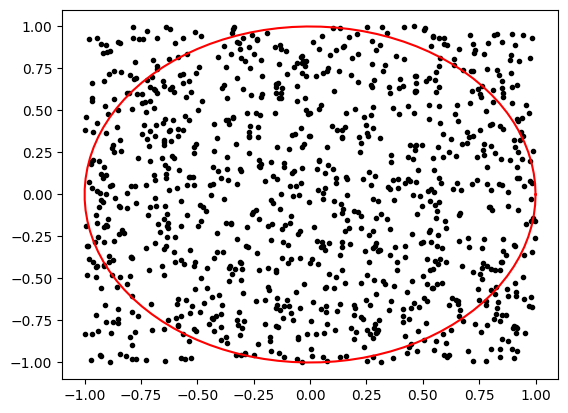
\includegraphics[width=.7\linewidth]{images/Figure1.png}
    \caption{}
    \label{fig:1}
\end{figure}
\begin{figure}[H]
    \centering
    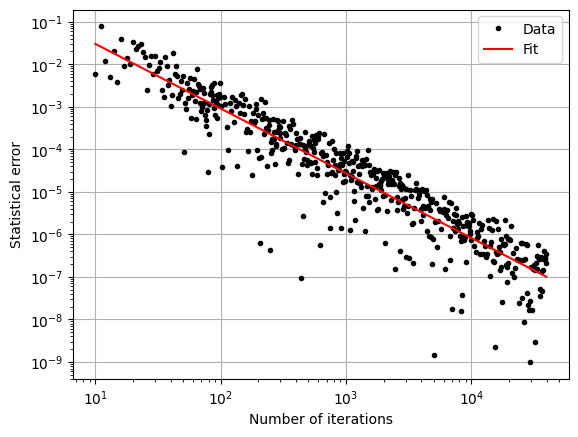
\includegraphics[width=.7\linewidth]{images/Figure1.2.png}
    \caption{log-log plot of the statistical error}
    \label{fig:1.1}
\end{figure}
\begin{figure}[H]
    \centering
    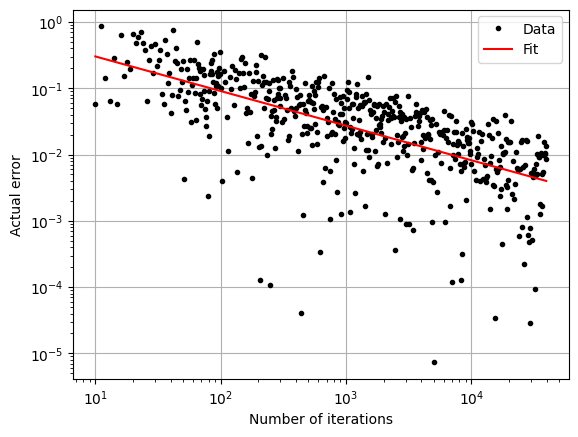
\includegraphics[width=.7\linewidth]{images/Figure1.1.png}
    \caption{log-log plot of the actual error}
    \label{fig:121}
\end{figure}
As we can see, it is confirmed that both statistical error and acutal error decrease as the number of iterations increases.
\clearpage
\section{Volume of a spere in 3D}
Consider a sphere of radius $R$, in three dimensions. We generate $N_{iter}$ random numbers using uniform random distribution, then we calculate the probability that point $(x,y,z)$ lies inside of the sphere and use it to approximate the volume of the sphere $V$ and compare it to the exact results: $V_{extact}=\frac43\pi R^3$.\\
As before report the statistical error $\sigma/\sqrt{N_{iter}}$ and compare it with the actual error, then make a log-log plot showing the statistical error and the actual error $|S-S_{exact}|$ as a function of the number of iterations.
\begin{equation}
    V\approx\frac{\text{Points inside the sphere}}{\text{Total number of points}}\times(2R)^3
\end{equation}
\begin{lstlisting}[language=Python]
Niter = 1000
p = 2*np.random.rand(Niter, 3)*R-R
Nhint = 0
for i in range(Niter):
    if p[i,0]**2 + p[i,1]**2 + p[i,2]**2 < R**2:
        Nhint += 1
        
V = (2*R)**3*Nhint/Niter
errAct = np.abs(V-4/3*np.pi*R**3)
errStat = np.sqrt((V-4/3*np.pi*R**3)**2/Niter**2)
\end{lstlisting}
\begin{lstlisting}
Using N: 1000 and D: 7
Estimated volume of the unit sphere: 4.256
Exact volume of the unit sphere: 4.1887902047863905
Actual error: 0.0672097952136097
Statistical error: 6.72097952136097e-05
\end{lstlisting}
\begin{figure}[H]
    \centering
    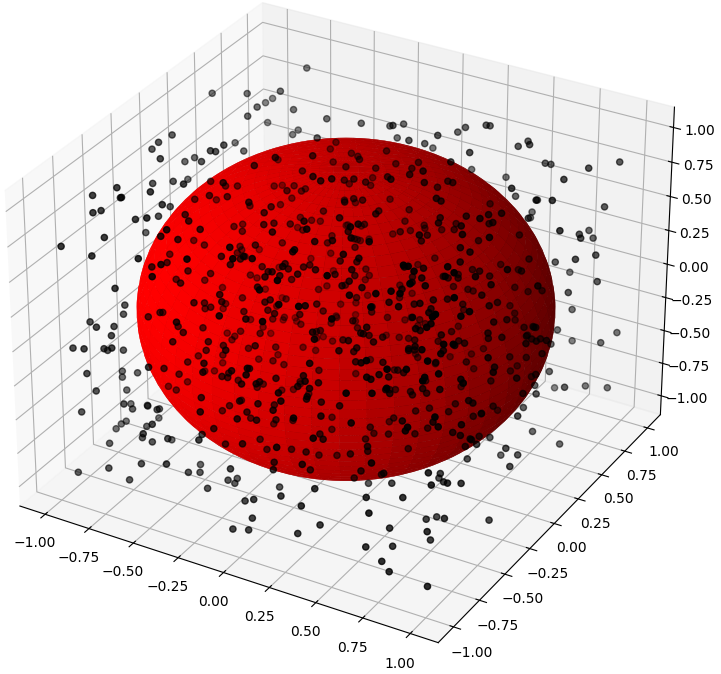
\includegraphics[width=.75\linewidth]{images/Figure2.png}
    \caption{}
    \label{fig:2}
\end{figure}
\begin{figure}[H]
    \centering
    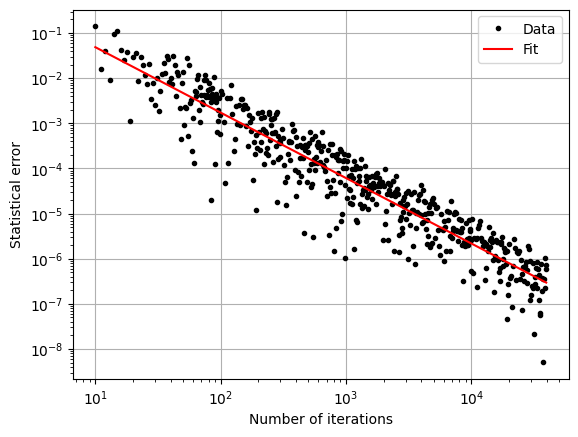
\includegraphics[width=.7\linewidth]{images/Figure2.1.png}
    \caption{log-log plot of the statistical error}
    \label{fig:2.1}
\end{figure}
\begin{figure}[H]
    \centering
    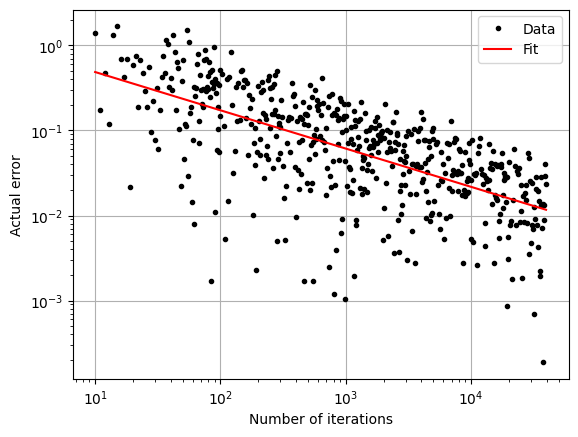
\includegraphics[width=.7\linewidth]{images/Figure2.2.png}
    \caption{log-log plot of the actual error}
    \label{fig:2.2}
\end{figure}
\clearpage
\section{Volume of a sphere in \textit{D} dimensions}
Now, we extend the concept to higher dimensions $D$. Similar to the sphere, the volume is estimated by calculating the fraction of points that fall within the hypersphere and then multiplying it by the volume of the hypercube that bounds the hypersphere.
\begin{equation}
    V\approx\frac{\text{Points inside hypersphere}}{\text{Total number of points}}\times(2R)^D
\end{equation}
and the exact result of the volume of an hypershere of radius $R$ in $D$ dimension is given by:
\begin{equation}\label{eq:volumehypersphere}
    V=\frac{\pi^{D/2}R^D}{\Gamma(D/2+1)}
\end{equation}
where $\Gamma$ is the gamma function.\\\\
We use the following code
\begin{lstlisting}[language=Python]
Niter = 10000
z = np.random.rand(Niter, D)
Nhint = 0
for i in range(Niter):
    if np.sum(z[i,:]**2) < 1:
        Nhint += 1
        
V = (2*R)**D*Nhint/Niter
Vth = np.pi**(D/2)*R**D/math.gamma(D/2+1)
errAct = np.abs(V-Vth)
errStat = np.sqrt((V-Vth)**2/Niter**2)
\end{lstlisting}
\begin{lstlisting}
Using N: 10000 and D: 7
Estimated volume of the unit hypersphere: 5.0304
Exact volume of the unit hypershpere: 4.7247659703314016
Actual error: 0.30563402966859865
Statistical error: 3.0563402966859864e-05
\end{lstlisting}
\begin{figure}[H]
    \centering
    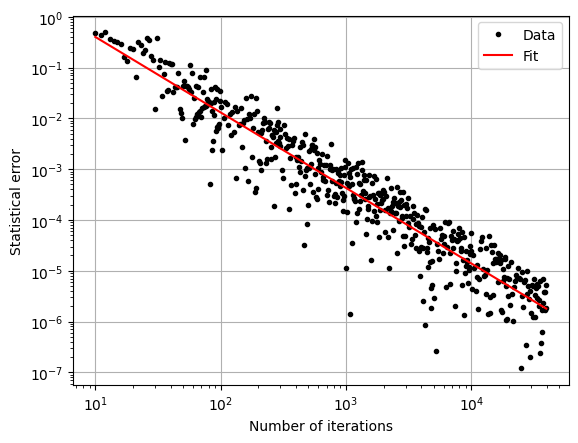
\includegraphics[width=.7\linewidth]{images/Figure3.2.png}
    \caption{log-log plot of the statistical error}
    \label{fig:3.2}
\end{figure}
\begin{figure}[H]
    \centering
    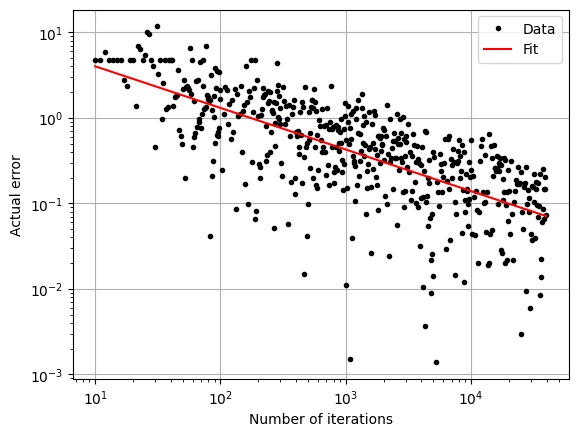
\includegraphics[width=.7\linewidth]{images/Figure3.1.png}
    \caption{log-log plot of the actual error}
    \label{fig:3.1}
\end{figure}
As we can observe, for low number of iterations the error is large.
\subsection{Hypersphere and hypercube}
The ratio between the volume of a sphere of diameter $2R$ and a cube with side length $2R$ in $D$ dimensions can be calculated as follows:
\begin{itemize}
    \item The volume of an hypersphere in $D$ dimension of radius $R$ is given by \autoref{eq:volumehypersphere}
    \item The volume of a hypercube in $D$ dimension with side $R$ is $R^D$
\end{itemize}
So we can compute the ratio
\begin{equation}
    \frac{\frac{\pi^{D/2}}{\Gamma(D/2+1)}(2R)^D}{(2R)^D}
\end{equation}
simplifying this, we find:
\begin{equation}
     \frac{\pi^{D/2}}{\Gamma(D/2+1)}
\end{equation}
It's worth noting that as $D$ increases, this ratio tends to zero rapidly, indicating that the hypersphere occupies a negligible portion of the hypercube's volume in higher dimensions.
\begin{figure}[H]
    \centering
    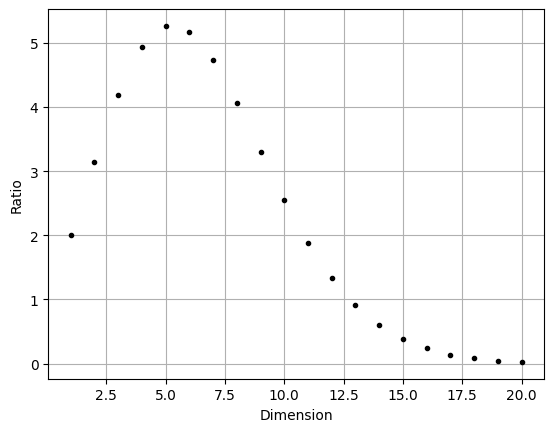
\includegraphics[width=.5\linewidth]{images/Figure4.png}
    \caption{plot of the ratio varying D}
    \label{fig:4}
\end{figure}
\end{document}